\chapter{Lösungskonzept}
\label{cha:Lösungskonzept}
Dieses Kapitel beschäftigt sich mit der Spezifikation des Vorlagenmanagements. Bei der Spezifikation handelt es sich um die Schnittstellen und die abstrakten Klassen, welche die Struktur des Vorlagenmanagements definieren und die gemeinsame Logik vorgeben. Diese Schnittstellen und abstrakten Klassen erlauben es, Implementierungen für verschiedene \emph{Template-Engines} zur Verfügung zu stellen wie z.B. für die
\begin{itemize}
	\item \emph{Template-Engine Freemakrer},
	\item \emph{Template-Engine Velocity} oder
	\item \emph{Template-Engine Thymeleaf}.
\end{itemize}
\ \newline
Mit der Möglichkeit, verschiedene \emph{Template-Engines} unterstützen zu können, soll das Vorlagenmanagement flexibel gehalten werden. Bei einem Wechsel zu einer anderen \emph{Template-Engine}, müssen nur die Ausdrücke in einer Vorlage in die \emph{Template-Engine}-spezifischen Ausdrücke konvertiert werden, was sich einfach realisieren lässt, da die Ausdrücke einer Vorlage immer gefunden werden müssen.

\section{Spezifikation des Vorlagenmanagements}
\label{sec:specification-template-management}
Dieser Abschnitt behandelt die Spezifikation des Vorlagenmanagements. Auf Basis dieser Spezifikation wird das Vorlagenmanagement und die Integration in die verschiedenen Umgebungen und Technologien implementiert. Diese Spezifikation ist frei von Abhängigkeiten auf konkrete Implementierungen jeglicher Art. Sie hat nur Abhängigkeiten auf andere Spezifikationen wie z.B. die \emph{JEE-7}-Spezifikation.
\newpage

\begin{figure}[h]
\centering
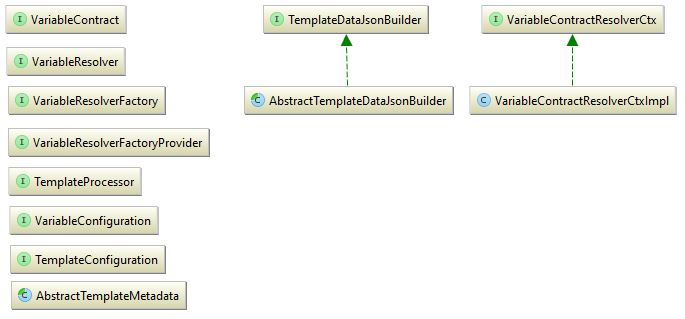
\includegraphics[scale=0.8]{20160710_template-logic-api.jpg} %{CS0031}
\caption{Klassenhierarchie des Vorlagenmanagements}
\label{fig:template-logic-api-hierarchy}
\end{figure}
\ \newline
Dieser Abschnitt behandelt die definierten Schnittstellen und abstrakten Klassen des Vorlagenmanagements. Die abstrakten Klassen implementieren die gemeinsam nutzbare Logik, die von allen konkreten Implementierungen des Vorlagenmanagements für jede \emph{Template-Engine} genutzt werden können. Die Schnittstellen und abstrakten Klassen aus Abbildung \ref{fig:template-logic-api-hierarchy}  spezifizieren die Aspekte des Vorlagenmanagements, wie
\begin{enumerate}
	\item das Variablenmanagement innerhalb des Vorlagenmanagement,
	\item die Handhabung von Variablen in einer Vorlage,
	\item die Abbildung der Metadaten einer Vorlage und 
	\item das Erstellen des \emph{JSON}-Datenobjekts, welches die serialisierten Daten der Variablen einer Vorlage, sowie die Metadaten der Vorlage, enthält.
\end{enumerate}

\subsubsection{Schnittstelle \emph{VariableContract}}
\label{sec:variableContract}
Die Schnittstelle \emph{VariableContract} aus dem Quelltext \ref{prog:variableContract} spezifiziert eine Variable, die in einer Vorlage verwendet werden kann. Objekte dieses Datentyps werden beim Anwendungsstart registriert und können grundsätzlich in allen Vorlagen verwendet werden. Eine Variable ist einem Modul zugeordnet, wobei die Variable bezüglich ihres Namens innerhalb des Moduls eindeutig sein muss. Das Modul wird über eine Zeichenkette definiert. Die Mehrsprachigkeit einer Variable wird über einen Aufzählungstyp realisiert, wobei jede Variable jeweils einen Schlüssel für die Bezeichnung und die Beschreibung bereit stellen muss.
\newline
\newline
Da es sich bei den Variablen um statische Daten handelt, also die Variablen schon beim Kompilieren bekannt sind, ist angedacht, dass die Variablen als eigener Aufzählungstyp implementiert werden, der die Schnittstelle \emph{VariableContract} implementiert. Durch die Abbildung der Variablen über einem eigenen Aufzählungstyp können mehrere Variablen in einer Klasse definiert werden, wobei jede einzelne Aufzählung des Aufzählungstyps ein Objekt des Datentyps \emph{VariableContract} darstellt. Alle Variablen, die mit einem eigenen Aufzählungstyp definiert werden, sollten demselben Modul zugeordnet sein, obwohl dies nicht zwingend erforderlich ist. Die Variablen, die mit einem Aufzählungstyp definiert wurden, werden innerhalb des Vorlagenmanagements trotzdem als einzelne Objekte des Datentyps  \emph{VariableContract} betrachtet. Die Tatsache dass die Variablen mit einem Aufzählungstyp abgebildet wurden, ist für das Vorlagenmanagement nur beim Registrieren der Variablen von Belang und nicht bei deren weiterer Verwendung.
\newline
\newline
Eine Variable ist über ihren Bezeichner global eindeutig identifizierbar, wobei sich der Bezeichner aus dem Modulnamen und dem Variablennamen zusammensetzt (Bsp. \emph{module.core.VAR\_1}). Der Bezeichner sowie der Modulname müssen sich an die Namenskonvention eines \emph{Java}-Paketnamens halten. Da der Variablenname immer auf diese Weise zusammengesetzt werden muss, wurde die Methode \emph{getId} als \emph{Default}-Methode implementiert, was seit Java 8 möglich ist. Ein(e) EntwicklerIn muss diese Methode nicht mehr implementieren, obwohl es immer noch möglich ist diese Methode zu überschreiben. Auch die Methode \emph{toInfoString} wurde als \emph{Default}-Methode implementiert, da auch diese Methode nicht von den EntwicklerInnen implementiert werden sollte, da ihre Funktionalität sich nicht ändern sollte.
\newline
\newline
[\cite[213]{java8InAction}] erklären \emph{Default}-Methoden wie folgt.
\begin{quote}
	\emph{Default methods are a new feature added in Java 8 to help evolve APIs in a compatible way. An interface can now contain method singatures for which an implementing class doesn't provide an implementation. So who implements them? The missing method bodies are given as part of the interface (hence default implementations) rather than in the implementing class. }
\end{quote}
\ \newline
Die Schnittstelle \emph{VariableContract} definiert \emph{Default}-Methoden nicht wegen einer Erweiterung der Schnittstelle, sondern wegen dem gleichen Verhalten der Methoden für alle Implementierungen.
\newpage

\begin{program}[h]
\caption{Die Schnittstelle \emph{VariableContract}}
\label{prog:variableContract}
\begin{JavaCode}
public interface VariableContract extends Serializable {

    String getName();

    String getModule();

    Enum<?> getInfoKey();

    Enum<?> getLabelKey();

    default String getId() {      
        return getModule() + "." + getName();
    }

    default String toInfoString() {
        final String        ls = System.lineSeparator();
        final StringBuilder sb = new StringBuilder();
        sb.append("contract  : ").append(this.getClass().getName())
          .append(ls)
          .append("id        : ").append(getId())
          .append(ls)
          .append("name      : ").append(getName())
          .append(ls)
          .append("label-key : ").append((getLabelKey() != null) 
                                          ? getLabelKey().name() 
                                          : "not available")
          .append(ls)
          .append("info-key  : ").append((getInfoKey() != null) 
                                          ? getInfoKey().name() 
                                          : "not available")
          .append(ls)
          .toString();
    }
    
}
\end{JavaCode}
\end{program}

\subsubsection{Schnittstelle \emph{VariableResolver}}
\label{sec:variableResolver}
Die Schnittstelle \emph{VariableResolver} aus dem Quelltext  \ref{prog:variableResolver} spezifiziert, wie der aktuelle Wert der Variablen ermittelt wird. 
\newline
\newline
Beim Erstellen einer \emph{E-Mail}-Nachricht auf Basis einer Vorlage müssen die aktuellen Werte der Variablen der Vorlage ermittelt werden. Da der aktuelle Wert einer Variable kontextabhängig ist, wird beim Ermitteln des aktuellen Werts einer Variable, ein Kontextobjekt bereitgestellt, über welche kontextabhängige Daten  bereitgestellt werden. Durch dieses Kontextobjekt, kann eine Variable in mehreren Kontexten verwendet werden und auch der aktuelle Wert einer Variable kontextabhängig ermittelt werden.
\begin{program}[h]
\caption{Die Schnittstelle \emph{VariableResolver}}
\label{prog:variableResolver}
\begin{JavaCode}
@FunctionalInterface
public interface VariableResolver {

    String resolve(VariableContract variable,
                   VariableContractResolverContext ctx);
                   
}
\end{JavaCode}
\end{program}
\ \newline
Die Schnittstelle \emph{VariableResolver} ist eine funktionale Schnittstelle, also einer Schnittstelle, die nur eine abstrakte Methode definiert, die implementiert werden muss. Eine Implementierung einer funktionale Schnittstelle kann auch über einen \emph{Lambda}-Ausdruck oder eine Methodenreferenz bereitgestellt werden, wodurch die Notwendigkeit einer anonymen Implementierung oder der Implementierung einer Klasse für diese Schnittstelle entfällt. Die Verwendung von \emph{Lambda}-Ausdrücken und Methodenreferenzen macht den Quelltext lesbarer, obwohl angemerkt sei, dass dieser Ansatz sich negativ auf das Laufzeitverhalten auswirkt, was in der Art und Weise der Ausführung eines \emph{Lambda}-Ausdrucks oder einer Methodenreferenz begründet ist. Die negativen Auswirkungen auf das Laufzeitverhalten können, in Bezug auf das Vorlagenmanagement, vernachlässigt werden. [\cite[50]{java8InAction}] beschreiben den Nutzen von funktionalen Schnittstellen wie folgt.
\begin{quote}
\emph{Functional interfaces are useful because the signature of the abstract method can describe the signature of a lambda expression. The signature of the abstract method of a functional interface is called a function descriptor.}
\end{quote}

\subsubsection{Schnittstelle \emph{VariableResolverFactory}}
\label{sec:variableResolverFactory}
Die Schnittstelle \emph{VariableResolverFactory} aus dem Quelltext  \ref{prog:variableResolverFactory} spezifiziert wie Objekte des Datentyps  \emph{VariableResolver} produziert werden. Objekte des Datentyps  \emph{VariableResolverFactory} können Objekte des Datentyps \emph{VariableResolver} für jede Implementierung der Schnittstelle \emph{VariableContract} produzieren. Es wird aber empfohlen, dass es je eine Implementierung der Schnittstelle \emph{VariableResolverFactory} je Modul gibt.
\newpage

\begin{program}
\caption{Die Schnittstelle \emph{VariableResolverFactory}}
\label{prog:variableResolverFactory}
\begin{JavaCode}
@FunctionalInterface
public interface VariableResolverFactory extends Serializable {

  VariableResolver getVariableResolver(VariableContract contract,
                                       VariableContractResolverCtx ctx);
                                       
}
\end{JavaCode}
\end{program}
\ \newline
Die Schnittstelle \emph{VariableResolver} ist eine funktionale Schnittstelle, damit Implementierungen über \emph{Lambda}-Ausdrücke oder Methodenreferenzen bereitgestellt werden können.

\subsubsection{Schnittstelle \emph{VariableResolverFactoryProvider}}
\label{sec:VariableResolverFactoryProvider}
Die Schnittstelle \emph{VariableResolverFactoryProvider} aus dem Quelltext  \ref{prog:variableResolverFactoryProvider} spezifiziert, wie Objekte des Datentyps  \emph{VariableResolverFacotry} produziert werden. Ein Objekt des Datentyps  \emph{VariableResolverFactoryProvider} kann Objekte des Datentyps  \emph{VariableResolverFactory} für die Schnittstelle \emph{VariableContract}, einer Ableitung von dieser Schnittstelle oder einer konkreten Implementierung dieser Schnittstelle zur Verfügung stellen. Die Schnittstelle \emph{VaraibleResolverFactoryProvider} wurde spezifiziert, damit in einer \emph{CDI}-Umgebung über ein Objekt dieses Datentyps die Objekte des Datentyps  \emph{VariableResolverFactory} produziert werden können, die von der \emph{CDI}-Umgebung zur Verfügung gestellt werden.

\begin{program}[h]
\caption{Die Schnittstelle \emph{VariableResolverFactoryProvider}}
\label{prog:variableResolverFactoryProvider}
\begin{JavaCode}
@FunctionalInterface
public interface VariableResolverFactoryProvider extends Serializable {

    VariableResolverFactory getVariableResolverFactory
            (Class<? extends VariableContract> contractType);
            
}
\end{JavaCode}
\end{program}
\ \newline
Die Schnittstelle \emph{VariableResolverFactoryProvider} ist ebenfalls eine funktionale Schnittstelle, damit Implementierungen über \emph{Lambda}-Ausrücke oder  Methodenreferenzen bereitgestellt werden können.

\subsubsection{Schnittstelle \emph{VariableContractResolverCtx}}
\label{sec:variableResolverFactoryProvider}
Die Schnittstelle \emph{VariableContractResolverCtx} aus dem Quelltext  \ref{prog:variableContractResolverCtx} spezifiziert den Kontext, der beim Ermitteln des aktuellen Werts einer Variable zur Verfügung gestellt wird. Dieser Kontext stellt alle Daten bereit, die beim Ermitteln des aktuellen Werts einer Variable benötigt werden. Es wird auch ermöglicht, dass Benutzerdaten im Kontext definiert werden können, die bei beim Ermitteln des aktuellen Werts einer Variable verwendet werden können. Es wurde bewusst vermieden, dass beim Ermitteln eines aktuellen Werts einer Variable bekannt ist, in welcher Vorlage die Variable verwendet wird. Dadurch bleibt die Handhabung der Variablen einer Vorlage entkoppelt von der Vorlage selbst. Dadurch wäre es z.B. auch möglich die Variablen außerhalb des Vorlagenmanagements zu verwenden.

\begin{program}[h]
\caption{Die Schnittstelle \emph{VariableContractResolverCtx}}
\label{prog:variableContractResolverCtx}
\begin{JavaCode}
public interface VariableContractResolverCtx {

    Locale getLocale();

    ZoneId getZoneId();

    TimeZone getTimeZone();

    <T> T getUserData(Object key, Class<T> clazz);
    
}
\end{JavaCode}
\end{program}

\subsubsection{Schnittstelle \emph{TemplateProcessor}}
\label{sec:templateProcessor}
Die Schnittstelle \emph{TemplateProcessor} aus dem Quelltext  \ref{prog:templateProcessor} spezifiziert, wie die Variablen in einer Vorlage behandelt werden. Objekte dieses Datentyps können Variablen in einer Vorlage für eine bestimmte \emph{Template-Engine} finden und konvertieren. Ein Objekt des Datentyps \emph{TemplateProcessor} muss in der Lage sein, ungültige Variablen innerhalb einer Vorlage zu finden, wobei eine ungültige Variable, eine Variable ist, die nicht registriert ist. Eine Implementierung der Schnittstelle \emph{TemplateProcessor} ist eine Implementierung für eine bestimmte \emph{Template-Engine}, da die in der Vorlage verwendeten Variablen, in Form von Ausdrücken spezifisch für die verwendete \emph{Template-Engine} sind. 
\newline
\newline
Der Quelltext \ref{prog:templateProcessor-highlighted-methods} zeigt die beiden Methoden der Schnittstelle \emph{TemplateProcessor}, die die Variablen in einer Vorlage konvertieren können.
\newpage

\begin{program}[h]
\caption{Die Methoden für die Konvertierung}
\label{prog:templateProcessor-highlighted-methods}
\begin{JavaCode}[numbers=none]
String replaceExpressions(
                  String template,
                  Function<VariableContract, String> converter);

String replaceCustom(String template,
                     Pattern itemPattern,
                     Function<String, String> converter);
\end{JavaCode}
\end{program}
\ \newline
Die Methoden aus dem Quelltext \ref{prog:templateProcessor-highlighted-methods} definieren als Formalparameter für den benötigte Konverter die funktionale Schnittstelle \emph{Function}, welche von Java 8 bereitgestellt wird. Dadurch ist das Spezifizieren einer eigenen Schnittstelle für die Konvertierung nicht mehr nötig. Der Konverter kann über einen \emph{Lambda}-Ausdruck oder Methodenreferenz bereitgestellt werden. Dadurch ist die Konvertierung der Variablen einer Vorlage abstrahiert von der Implementierung der Schnittstelle \emph{TemplateProcessor}, wodurch die Variablen durch eine beliebige Repräsentation ersetzt werden können.

\begin{program}[h]
\caption{Die Schnittstelle \emph{TemplateProcessor}}
\label{prog:templateProcessor}
\begin{JavaCode}
public interface TemplateProcessor {

    String replaceExpressions(
                      String template,
                      Function<VariableContract, String> converter);

    String replaceCustom(String template,
                         Pattern itemPattern,
                         Function<String, String> converter);

    Set<VariableContract> resolveExpressions(String template);

    Set<String> resolveInvalidExpressions(String template);

    String variableToExpression(VariableContract contract);

    VariableContract expressionToVariable(String expression);
    
}
\end{JavaCode}
\end{program}

\subsubsection{Schnittstelle \emph{TemplateDataJsonBuilder}}
\label{sec:templateDataJsonBuilder}
Die Schnittstelle \emph{TemplateDataJsonBuilder} aus dem Quelltext  \ref{prog:templateDataJsonBuilder} spezifiziert die Signatur eines \emph{Builders}, der das Datenobjekt erstellt, welches die Daten für das Ausprägen einer Vorlage enthält. Das erstellte Datenobjekt enthält die folgenden Daten:
\begin{itemize}
	\item Die Sprache, in der die Vorlage erstellt wurde,
	\item die Zone für die Konvertierung von Datums- und Zeitwerten,
	\item die Version der Vorlage und 
	\item die Metadaten der Vorlage wie z.B die Anzahl der enthaltenen Variablen.
\end{itemize} 
Das Datenobjekt kann in den folgenden Repräsentationen vom \emph{Builder} bereitgestellt werden:
\begin{itemize}
	\item Als \emph{Java}-Objekt,
	\item als \emph{JSON}-Zeichenkette oder
	\item als Objekt der Klasse \emph{java.util.Map}.
\end{itemize}
\ \newline
Anstelle der Serialisierung der Daten könnte die Vorlage auch ausgeprägt und persistent gehalten werden, wodurch aber die Menge an persistent gehaltenen Daten stark ansteigen würde. Mit dem Datenobjekt werden nur die benötigten Daten persistent gehalten, wodurch die Menge an persistent gehaltenen Daten so klein wie möglich gehalten wird. Mit dem Datenobjekt kann die korrespondierende Vorlage zu jedem Zeitpunkt mit demselben Resultat wiederhergestellt werden.
\newline
\newline
Es wurde das Entwurfsmuster \emph{Builder} [\cite[97]{designPatterns}] verwendet, da sich die Konfiguration des \emph{Builders} mit einer \emph{Fluent}-Schnittstelle [\cite{fowlerFluentInterface}], wie bei einem \emph{Builder} üblich, sehr gut abbilden lässt. Die Schnittstelle \emph{TemplateDataJsonBuilder} spezifiziert folgende Terminalmethoden.
\begin{itemize}
	\item\emph{TemplateRequestJson toJsonModel()} liefert das Datenobjekt in Form eines \emph{Java}-Objekts.
	\item\emph{String toJsonString()} liefert das Datenobjekt als \emph{JSON}-Zeichenkette.
	\item\emph{Map<String, Object> toJsonMap()} liefert das Datenobjekt in Form eines Objekts der Klasse \emph{java.util.Map}.
\end{itemize} 
\ \newpage

\begin{program}
\caption{Die Schnittstelle \emph{TemplateDataJsonBuilder}}
\label{prog:templateDataJsonBuilder}
\begin{JavaCode}
public interface TemplateDataJsonBuilder<
    I,
    M extends AbstractTemplateMetadata<I>,
    B extends TemplateDataJsonBuilder> extends Serializable {

    B withWeakMode();

    B withLocalization(Locale locale,
                       ZoneId zoneId);

    B withUserData(Map<Object, Object> userData);

    B withStrictMode();

    B withVariableResolverFactoryProvider
                         (VariableResolverFactoryProvider factory);

    B withVariableResolverFactory(VariableResolverFactory factory);

    B withTemplate(M metadata);

    B addVariable(VariableContract contract, Object value);

    B addVariableResolver(VariableContract contract,
                          VariableResolver resolver);

    TemplateRequestJson toJsonModel();

    String toJsonString();

    Map<String, Object> toJsonMap();
    
}
\end{JavaCode}
\end{program}
\ \newline 
[\cite[100]{designPatterns}] beschreiben die Implementierung eines \emph{Builders} wie folgt:
\begin{quote}
\emph{Typically there's an abstract Builder class that defines an operation for each component that a director may ask it to create. The operations do nothing by default. A ConcreteBuilder class overrides operations for components it's interested in creating.}
\end{quote}
[\cite[96 - 106]{designPatterns}] beschreiben ausführlich das Entwurfsmuster \emph{Builder}, jedoch ohne die Verwendung einer \emph{Fluent}-Schnittstelle, die heutzutage über den \emph{Builder} gelegt wird, um dessen Anwendung über Punktnotation angenehmer zu machen. Mit einer \emph{Fluent}-Schnittstelle wird die Möglichkeit geboten, einzelne Komponenten des zu bauenden Objektes zu setzen. Der Quelltext \ref{prog:templateDataJsonBuilder-example} zeigt, wie der \emph{Builder} des Datentyps \emph{TemplateDataJsonBuilder} mit einer \emph{Fluent}-Schnittstelle verwendet wird.

\begin{program}[h]
\caption{Beispiel der Anwendung des \emph{Builders}}
\label{prog:templateDataJsonBuilder-example}
\begin{JavaCode}
TemplateDataJsonBuilder builder;
TemplateRequestJson     model;

builder = new TemplateDataJsonBuilderImpl();
model   = builder.withStrictMode() 
               .withLocalization(localeObj, zoneIdObj)
               .withTemplate(templateMetadataObj)
               .withUserData(userDataMap)
               .withVariableResolverFactoryProvider(factoryProviderObj)
               .toJsonModel();
\end{JavaCode}
\end{program}

\subsubsection{Abstrakte Klasse \emph{AbstractTemplateMetadata}}
\label{sec:abstractTemplateMetadata}
Die abstrakte Klasse \emph{AbstractTemplateMetadata} implementiert die Logik, die von allen konkreten Ableitungen dieser abstrakten Klasse für die verschiedenen \emph{Template-Engines} genutzt werden kann. Metadaten wie
\begin{itemize}
	\item die Anzahl der gültigen Variablen in der Vorlage,
	\item die Anzahl der nicht registrierten Variablen in der Vorlage,
	\item die Zeichenanzahl der Vorlage,
	\item der eindeutige Bezeichner der Vorlage,
	\item die Version der Vorlage und
	\item die Vorlage selbst,  
\end{itemize}
werden in dieser Klasse abgebildet.
\newline
Diese Metadaten sind unabhängig von der verwendeten \emph{Template-Engine} und eine Implementierung für eine spezifische \emph{Template-Engine} kann zusätzliche Metadaten definieren. Die Metadaten werden einmalig ermittelt und sind über die Lebenszeit des Objekts des Datentyps \emph{AbstractTemplateMetadata} unveränderbar. Wird die Vorlage geändert so muss das Objekt der Metadaten entweder neu erstellt oder neu initialisiert werden.

\subsubsection{Abstrakte Klasse \emph{AbstractTemplateDataJsonBuilder}}
\label{sec:abstractTemplateDataJsonBuilder}
Die abstrakte Klasse \emph{AbstractTemplateDataJsonBuilder} implementiert die gemeinsam nutzbare Logik, die von allen konkreten Ableitungen für die verschiedenen \emph{Template-Engines} verwendet werden kann. Sie stellt Hilfsmethoden bereit, die Variablen innerhalb der Vorlage finden, validieren und den aktuellen Wert von Variablen ermitteln können. Das resultierende Datenobjekt des \emph{Builders} ist spezifiziert, jedoch nicht die Abbildung der ermittelten Werte für die enthaltenen Variablen. Diese Daten sind spezifisch für die verwendete \emph{Template-Engine}.

\section{Spezifikation der Vorlagenintegration}
Die im Abschnitt \ref{sec:specification-template-management} vorgestellte Spezifikation des Vorlagenmanagements, spezifiziert die Kernfunktionalität des Vorlagenmanagements, das in der Lage ist die Vorlagen sowie deren enthaltene Variablen zu behandeln. Das Vorlagenmanagement benötigt auch Integrationen in verschiedene Umgebungen und Sprachen, um die benötigte Funktionalitäten wie
\begin{itemize}
	\item die Verwaltung der Variablen im  \emph{JavaScript}-basierten \emph{CKEditor},
	\item die automatische Registrierung der Variablen in einer \emph{CDI}-Umgebung,
	\item die Verwaltung der Vorlagen über eine Webseite und
	\item die Persistenz der Vorlagen realisieren zu können. 
\end{itemize}
\ \newline
Folgender Abschnitt behandelt die Spezifikation der Integrationen wie in Abschnitt \ref{sec:technical-goals} vorgegeben. 
 
\subsection{Vorlagenmanagement in \emph{TypeScript}}
\label{sec:sub-typescript-javascript}
Wie in Abschnitt \ref{sec:sub-template-management-website} vorgegeben, muss der \emph{JavaScript}-basierte \emph{Editor CKEditor} verwendet werden, mit dem \emph{HTML} basierte Vorlagen über eine Webseite bearbeitet werden können. Der \emph{CKEditor} muss angepasst werden, damit die definierten Variablen in einer Vorlage verwendet werden können. Es wird ein \emph{CKEditor-Plugin} in \emph{TypeScript} entwickelt, das es erlaubt, die definierten Variablen innerhalb des \emph{CKEditors} und dessen enthaltener Vorlage zu verwalten. Es wird die Skriptsprache \emph{TypeScript} verwendet, da es mit dieser Skriptsprache möglich ist typsicher zu entwickeln, was in \emph{JavaScript} nicht möglich ist. Ebenfalls kann \emph{TypeScript} in mehrere \emph{ECMA}-Standards übersetzt werden.
\newline
\newline
Innerhalb des \emph{CKEditor-Plguins} werden Variablen verwendet, dessen Management in einer eigenen Quelltextdatei implementiert wird, da das Variablenmanagement unabhängig vom \emph{CKEditor-Plguin} ist und daher auch anderweitig verwendet werden kann. Damit wird das Variablenmanagement entkoppelt vom \emph{CKEditor-Plugin} sein.

\subsection{Vorlagenmanagement in \emph{CDI}}
\label{sec:sub-template-management-cdi}
Das Vorlagenmanagement wird in einem \emph{JEE-7}-Anwendungsserver verwendet werden, der eine \emph{CDI}-Umgebung bereitstellt. Im \emph{CDI}-Standard sind portable Erweiterungen  spezifiziert, die es erlauben, dass sich Softwarekomponenten in einer \emph{CDI}-Umgebung integrieren können. Es wird eine \emph{CDI}-Erweiterung implementiert, die beim Start der \emph{CDI}-Erweiterung, die definierten Variablen automatisch registriert und über den Lebenszyklus der Anwendung persistent hält. Es werden Objekte des Vorlagenmanagements wie z.B
\begin{itemize}
	\item Objekte der Schnittstelle \emph{VariableResolver},
	\item Objekte der Schnittstelle \emph{VariableResolverFactory} oder
	\item Objekte der Schnittstelle \emph{TemplateDataJsonBuilder} kontextabhängig zur Verfügung gestellt.
\end{itemize}
\ \newline
Durch die Verwaltung der Objekte von einer \emph{CDI}-Umgebung, können sich Implementierungen der Schnittstelle \emph{VariableResolver} kontextabhängige Ressourcen injizieren lassen. Damit das Variablenmanagement auf diese Objekte zugreifen kann, wurde die Schnittstelle \emph{VariableResolverFactoryProvider} spezifiziert, die die Verbindung des Variablenmanagements zu einer \emph{CDI}-Umgebung herstellt und kontextabhängige Objekte der Schnittstelle \emph{VariableResolverFactory} bereitstellen kann.

\subsection{Vorlagenmanagement in \emph{JSF}}
\label{sec-sub-specification-jsf}
Für die Verwaltung der Vorlagen wird eine \emph{JSF}-Webseite implementiert. Über diese Webseite können Vorlagen erstellt, modifiziert und gelöscht werden. Für die Verwaltung der Vorlagen wird die von \emph{PrimeFaces-Extension} bereitgestellte \emph{JSF}-Komponente für den \emph{Editor CKEditor} verwendet. Diese Komponente integriert den \emph{JavaScript}-basierten \emph{CKEDitor} in den \emph{JSF}-Lebenszyklus. Um die Vorlage in die korrespondierende \emph{Template-Engine} spezifische Repräsentation zu überführen, wird ein \emph{FacesConverter} implementiert, der die Konvertierung der Vorlage von seiner Repräsentation in \emph{HTML} in die \emph{Template-Engine} spezifische Repräsentation und visa versa ermöglicht.

\subsection{Vorlagenmanagement im \emph{Mail}-DB-Schema}
Eine Vorlage wird durch eine Zeichenkette repräsentiert, die innerhalb des \emph{Mail}-DB-Schema sprachspezifisch  persistent gehalten wird. Es ist nicht erforderlich eine eigene Tabellenstruktur für die Vorlagen zu definieren um es von den \emph{Mail}-Tabellen zu abstrahieren, da die Vorlagen einen essentiellen Teil von \emph{CleverMail} darstellen und daher auch die Vorlagen bzw. deren persistente Repräsentation voll in das \emph{Mail}-DB-Schema  integriert werden müssen. Sollten die Vorlagen außerhalb von \emph{CleverMail} verwendet werden so kann dies leicht realisiert werden, da eine Vorlage nur eine Zeichenkette darstellt, die einfach persistent gehalten werden kann.